\documentclass[man,floatsintext]{apa6}
\usepackage{lmodern}
\usepackage{amssymb,amsmath}
\usepackage{ifxetex,ifluatex}
\usepackage{fixltx2e} % provides \textsubscript
\ifnum 0\ifxetex 1\fi\ifluatex 1\fi=0 % if pdftex
  \usepackage[T1]{fontenc}
  \usepackage[utf8]{inputenc}
\else % if luatex or xelatex
  \ifxetex
    \usepackage{mathspec}
  \else
    \usepackage{fontspec}
  \fi
  \defaultfontfeatures{Ligatures=TeX,Scale=MatchLowercase}
\fi
% use upquote if available, for straight quotes in verbatim environments
\IfFileExists{upquote.sty}{\usepackage{upquote}}{}
% use microtype if available
\IfFileExists{microtype.sty}{%
\usepackage{microtype}
\UseMicrotypeSet[protrusion]{basicmath} % disable protrusion for tt fonts
}{}
\usepackage{hyperref}
\hypersetup{unicode=true,
            pdftitle={Understanding order effects in word learning},
            pdfauthor={George Kachergis, Daniel Yurovsky, \& Michael C. Frank},
            pdfkeywords={cross-situational word learning; order effects; spacing; temporal contiguity},
            pdfborder={0 0 0},
            breaklinks=true}
\urlstyle{same}  % don't use monospace font for urls
\usepackage{graphicx,grffile}
\makeatletter
\def\maxwidth{\ifdim\Gin@nat@width>\linewidth\linewidth\else\Gin@nat@width\fi}
\def\maxheight{\ifdim\Gin@nat@height>\textheight\textheight\else\Gin@nat@height\fi}
\makeatother
% Scale images if necessary, so that they will not overflow the page
% margins by default, and it is still possible to overwrite the defaults
% using explicit options in \includegraphics[width, height, ...]{}
\setkeys{Gin}{width=\maxwidth,height=\maxheight,keepaspectratio}
\IfFileExists{parskip.sty}{%
\usepackage{parskip}
}{% else
\setlength{\parindent}{0pt}
\setlength{\parskip}{6pt plus 2pt minus 1pt}
}
\setlength{\emergencystretch}{3em}  % prevent overfull lines
\providecommand{\tightlist}{%
  \setlength{\itemsep}{0pt}\setlength{\parskip}{0pt}}
\setcounter{secnumdepth}{0}
% Redefines (sub)paragraphs to behave more like sections
\ifx\paragraph\undefined\else
\let\oldparagraph\paragraph
\renewcommand{\paragraph}[1]{\oldparagraph{#1}\mbox{}}
\fi
\ifx\subparagraph\undefined\else
\let\oldsubparagraph\subparagraph
\renewcommand{\subparagraph}[1]{\oldsubparagraph{#1}\mbox{}}
\fi

%%% Use protect on footnotes to avoid problems with footnotes in titles
\let\rmarkdownfootnote\footnote%
\def\footnote{\protect\rmarkdownfootnote}


  \title{Understanding order effects in word learning}
    \author{George Kachergis\textsuperscript{1}, Daniel Yurovsky\textsuperscript{2}, \& Michael C. Frank\textsuperscript{1}}
    \date{}
  
\shorttitle{Order effects in word learning}
\affiliation{
\vspace{0.5cm}
\textsuperscript{1} Department of Psychology, Stanford University\\\textsuperscript{2} Department of Psychology, Carnegie Mellon University}
\keywords{cross-situational word learning; order effects; spacing; temporal contiguity\newline\indent Word count: 111}
\usepackage{csquotes}
\usepackage{upgreek}
\captionsetup{font=singlespacing,justification=justified}

\usepackage{longtable}
\usepackage{lscape}
\usepackage{multirow}
\usepackage{tabularx}
\usepackage[flushleft]{threeparttable}
\usepackage{threeparttablex}

\newenvironment{lltable}{\begin{landscape}\begin{center}\begin{ThreePartTable}}{\end{ThreePartTable}\end{center}\end{landscape}}

\makeatletter
\newcommand\LastLTentrywidth{1em}
\newlength\longtablewidth
\setlength{\longtablewidth}{1in}
\newcommand{\getlongtablewidth}{\begingroup \ifcsname LT@\roman{LT@tables}\endcsname \global\longtablewidth=0pt \renewcommand{\LT@entry}[2]{\global\advance\longtablewidth by ##2\relax\gdef\LastLTentrywidth{##2}}\@nameuse{LT@\roman{LT@tables}} \fi \endgroup}


\usepackage{lineno}

\linenumbers
\usepackage{float}

\authornote{

Correspondence concerning this article should be addressed to Michael C. Frank, Stanford, CA 94305 USA. E-mail: \href{mailto:mcfrank@stanford.edu}{\nolinkurl{mcfrank@stanford.edu}}}

\abstract{
hazy indefinite words outline


}

\begin{document}
\maketitle

\hypertarget{introduction}{%
\section{Introduction}\label{introduction}}

In order to learn a language, learners must rely on others to occasionally mention objects in their shared environment.
However, it may not be clear to the learner exactly which object a speaker is naming at any given moment.
The learner may disambiguate which words refer to which objects if names co-occur most frequently with their intended referents, and the learner remembers frequent word-object pairings.
Such cross-situational learning (Gleitman, 1990) does not even rely on every correct pairing appearing more frequently than others, since learners employ a mutual exclusivity bias---one word for each object, demonstrated in toddlers (Markman \& Wachtel, 1988)--to effectively infer word-object mappings that are completely correlated with other pairs ({\textbf{???}}).

In the cross-situational word learning paradigm (Smith \& Yu, 2008), a learner acquires word meanings by tracking the co-occurrences words and objects across situations containing several words and objects.
For example, adults are presented with a series of study trials, each displaying four uncommon objects (e.g., an abstract sculpture) while four pseudowords are spoken (e.g., \enquote{manu}, \enquote{bosa}).
Although each pseudoword refers to an onscreen object, the intended referent is not indicated, leaving the correct pairings on each trial quite ambiguous.
With this trial configuration, when given a total of 18 word-object pairs across 27 trials---yielding 6 repetitions per pair---the average adult learner adult learner chooses the correct object for each word from 3 other objects (i.e., 4AFC testing) for 9.5 of the 18 pairs.

Given perfect knowledge of which words and objects appeared on each trial, and perfect discrimination among the words and objects, myriad simple algorithms can perform this task.
For example, maintaining a word x object co-occurrence count matrix and choosing the most frequent object for each word guarantees flawless performance.
However, such a strategy requires accurately storing and retrieving an 18x18 matrix of counts--an unlikely feat for human memory.
Instead, human learners likely select and store a subset of the word-object co-occurrences on each trial, perhaps on the basis of what is noisily remembered from preceding trials.
For example, if words \{w1, w2, w3, w4\} and objects \{o1, o2, o3, o4\} appeared on the first trial, and \{w1, w5, w6, w7\} and \{o1, o5, o6, o7\} were presented on the next trial, learners may realize that pair 1 (i.e., w1-o1) was repeated, and devote more attention to storing this association than to the still-ambiguous word-object pairings (i.e., pairs 5-7).
Assuming that influences from such trial-to-trial contiguity are present, Yu and Smith (2007) and many other previous studies {[}XXX{]} did not allow such contiguities: pairs were forbidden from appearing in consecutive trials.

However, such repetitions are common in real learning environments, in part because the physical environment is often temporally contiguous: objects do not spontaneously disappear, to be replaced by new objects.
Rather, both situations and topics of conversation may gradually evolve over time, with objects and topics being replaced bit by bit as one passes from one room to the next.
Such temporal contiguity can aid learning in more than one situation.
As illustrated above, repeating a word-object pair in two consecutive trials can allow inference of the repeated pair, assuming memory for first trial.
Similarly, consider two successive trials on which three of the four word-referent pairs are repeated: \{w1, w2, w3, w4; o1, o2, o3, o4\} followed by \{w1, w2, w3, w5; o1, o2, o3, o5\}.
In this case, if \emph{w5} and \emph{o5} can be identified as the unrepeated stimuli then the learner may infer that they are linked.
Thus, a single unrepeated pair might be as useful for learning as a single repeated pair.

However, in both of these examples, temporal contiguity may not only confer an advantage for the single pair that can be inferred: if a learner can indeed separate repeated from unrepeated stimuli, this will also reduce---though not eliminate---the ambiguity of the larger subset of stimuli, since repeated words should refer to repeated objects, and unrepeated words to unrepeated objects.
hus, in the case of one repeated pair, the three unrepeated pairs (5-7) form only 9 possible pairings, whereas a trial with no repeated (or all repeated) stimuli contains 16 possible pairings.
With three repeated pairs, the situation is the same.
Hence, temporal contiguity might help not only by allowing direct inference of single pairs, but also by reducing the complexity of the learning problem--but only if learners can indeed separately associate repeated and unrepeated stimuli.

In the following studies we assess the effects of different degrees of temporal contiguity and model the results. In Experiment 1, we simply shuffle trials to achieve different degrees of successive repetitions.
In Experiment 2, we test specific types of trial-to-trial repetitions to better discern the effects.
Finally, we introduce an intuitive extension to a cross-situational word learning model ({\textbf{???}}) that captures the main findings.

\hypertarget{experiment-1}{%
\section{Experiment 1}\label{experiment-1}}

In this cross-situational word learning study we investigate the effects on learning of repeating some word-object pairs on successive trials.
As discussed above, the degree of overlap between two trials may reasonably facilitate learning in different ways: repeating a single pair--or all but one of the pairs--allows inference of the unique pair, but may also improve learning of the remaining pairs by reducing the number of conceivable pairings.
But in the extreme, too much trial-to-trial repetition may become monotonous or even uninformative.
In general, it is expected that trial orderings with more trial-to-trial repetitions will yield higher overall learning.

Each training block consisted of sequences of 27 trials, during which 18 pseudoword-object pairs were presented six times (correct pairs co-occurring six times; spurious word-object co-occurrences ranged from 0 to 4, M = 1.5).
The control condition was a fixed temporal sequence containing no pairs that repeated on successive trials, taken from Kachergis, Yu, and Shiffrin (2016).
In all of the other conditions, the individual training trials were the same set used in this control condition.
However, the order of the trials was shuffled many times to create orderings with degrees of trial-to-trial repetitions.
Because the orderings were all constructed from the same set of trials, all co-occurrence statistics remained identical across conditions.

The successive repetition (SR) score of a sequence of training trials is the mean number of word-referent pairings that overlap across all consecutive pairs of trials.
The minimum SR score is 0, as no pairs ever overlap.
A single trial repeated 27 times would yield a maximal SR score of 4, but of course this is not a reasonable learning situation.
The maximum SR score we were able to obtain by reshuffling the control sequence was 2.04, meaning that in this condition, on average, slightly more than two word-referent pairs repeated in every pair of successive trials.
The training trial sequences we constructed and used had SR scores of 0.00, 0.33, 0.67, 1.00, 1.41, and 2.04.

Assuming memory of the preceding trial, repeating some of the pseudoword-referent pairs from trial \emph{n-1} on trial \emph{n} allows segregation of possible pairings into two subgroups -- repeated pairs and unrepeated pairs -- perhaps as a result of attention being drawn to the repeated stimuli.
Such segregation of a large set with many possible pairings (i.e., 4×4 = 16) into two smaller subsets with a fewer total number of pairings (i.e., 2×2 + 2×2 = 8) reduces ambiguity, so it was expected that conditions with higher SR scores would result in increased learning.

\hypertarget{method}{%
\subsection{Method}\label{method}}

\hypertarget{participants}{%
\subsubsection{Participants}\label{participants}}

Participants were undergraduates at Indiana University who received course credit for participating.
There were 76 participants in condition SR = 0--a control condition used in many experiments; 36 in conditions SR = \{.33, .66, 1.0, and 1.41\}; and 31 in condition SR = 2.04.

\hypertarget{stimuli}{%
\subsubsection{Stimuli}\label{stimuli}}

Stimuli are 48 images of unusual objects (e.g., sculptures) and 48 spoken pseudowords. The pseudowords are computer-generated, phonotactically-probable in English (e.g., \enquote{bosa}), and pronounced by a monotone, synthetic female voice.

On each training trial, pictures of four uncommon objects (e.g., a metal sculpture) were simultaneously shown while four spoken pseudowords were serially played.
The 72 computer-generated pseudowords are phonotactically-probable in English (e.g., \enquote{bosa}), and were spoken by a synthetic, monotone female voice.
The 72 words and 72 objects were randomly assigned to four sets of 18 word-object pairings.
On each training trial, the four pictures appeared immediately. After two seconds of initial silence, each pseudoword was played for one second with two seconds of silence between pseudowords, for a total trial duration of 12 seconds.
The pseudowords on each trial were presented in random order.
Each training sequence consisted of 27 such trials, with each \enquote{correct} pseudoword-object mapping occurring 6 times, and other mappings occurring from 0 to 4 times (M=1.5).
Upon completion of each training phase, participants were tested for their knowledge of the \enquote{correct} (i.e.~most frequently co-occurring) pairings.
On each test trial, a single pseudoword was played and all 18 objects were displayed.
Participants were asked to click on the correct object for that pseudoword.
Each pseudoword was tested once, and the test order was randomized for each participant and condition.
Participants completed four pairs of training/test blocks in a randomized order.

\hypertarget{procedure}{%
\subsubsection{Procedure}\label{procedure}}

Participants were instructed that they would see a series of trials with objects and alien words, and that they should try to figure out what each word means for a final test.
After training, their knowledge was assessed using 18-alternative forced choice (18AFC) testing: on each test trial a single word was played, and the participant was instructed to choose the appropriate object from a display of the 18 trained referents.

\hypertarget{results}{%
\subsection{Results}\label{results}}

Figure 1 shows the overall performance achieved in each condition of Experiment 1. Increasing the degree of successive repetitions does produce increased performance, as predicted, showing a strong correlation. However, the increases are surprisingly modest relative to what might have been expected a priori. For detailed analysis of each condition, to-be-learned pairs were grouped according to the number of times they had successive repetitions in the sequence (see Table 1). Surprisingly, the relation between performance and SR was often non-monotonic. For example, consider the trial ordering with mean SR = 1.0. In this condition, the non-repeated pairs were learned with 45\% accuracy, the pairs that overlapped once were learned with only 30\% accuracy, and the pairs that overlapped three times were learned with 66\% accuracy. In some other conditions, performance was more or less equal for all degrees of repetition. Only in the two conditions of low SR (SR=.33 and SR=.67) did greater successive repetition confer a modest learning advantage.

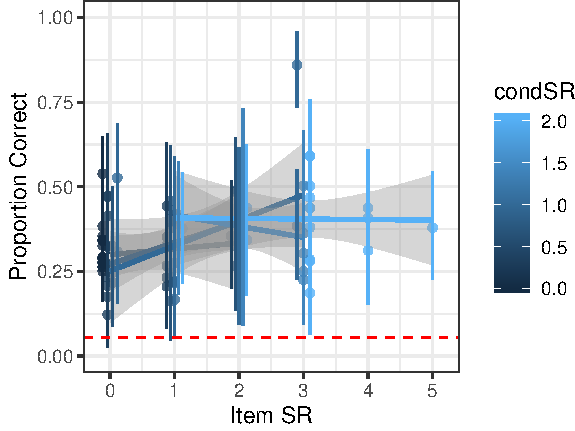
\includegraphics{figs/fig1-exp1-1.pdf}
Figure 1: Accuracy (18AFC; chance=.056) for conditions with varying degrees of average successive repetitions (SR). Greater mean SR in a condition tended to improve learning performance, although not as drastically as expected. Error bars are +/-SE.

These results show that learning is increased by increasing the average degree of successive repetitions, even while leaving all within-trial co-occurrence statistics constant. However, based on the detailed analysis in Table 1, it is clear that this learning increase was not simply due to increased learning for successively repeated pairs. For instance, in the SR=1.0 condition, non-repeated pairs were learned better than 1- and 2-repetition pairs. The difficulty of learning a given pair is not solely due to the number of successive repetitions for that pair in a sequence. Perhaps the presence of other repeated pairs interfered with the learning of a given pair. Another relevant factor may be the interaction of spacing and sequential effects: for each case where a pair occurs in successive trials, that pair will appear one fewer time later in training (since each pair only appeared 6 times during training).

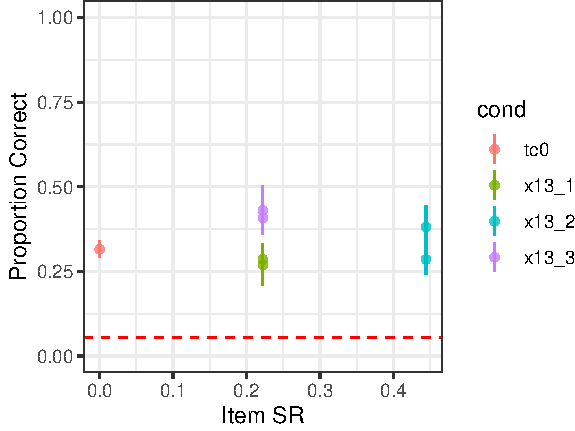
\includegraphics{figs/exp2-1.pdf}

\hypertarget{experiment-2}{%
\section{Experiment 2}\label{experiment-2}}

Experiment 1 showed that increasing the mean successive repetitions in a trial ordering facilitates learning for the entire set of pairings, but that greater numbers of successive repetitions does not always confer an advantage for the repeated pairs. Instead, learning of unrepeated pairs seems to improve with the presence of greater overall successive repetitions in the condition. To better understand the role that successive repetitions can play in statistical learning of both repeated and unrepeated pairs, we implemented three different types of temporal contiguity in three sequences of 27 training trials, exemplified in Table 2. In the 1 pair/2 trials condition, 9 of the 18 pairs appeared in two consecutive trials at some point during the training. In the 1 pair/3 trials condition, 9 of the 18 pairs appeared in three consecutive trials. Importantly, in both of these conditions, no other stimuli in the overlapping trials simultaneously overlapped. In the 2 pairs/2 trials condition, however, each of the 18 pairs at some point appeared with another pair in two consecutive trials.

Importantly, these conditions offer different ways to perform inferences and consequently reduce the degree of ambiguity. For example, consider just two successive trials with one pair only repeated, as in the 1 pair/2 trials condition. The repeated pair may be immediately inferred to be correct, but the remaining six pairs on the two trials remains ambiguous---there are still 9 possible pairings for each of the three remaining words and objects in each trial. For another example, when two pairs are repeated in two successive trials, as in the 2 pairs/2 trials condition, no pairing can be unambiguously inferred. However, overall ambiguity is considerably reduced: If (A B X Y; b a y x) occurred on trial n, and (A B E F; a b e f) occurred on trial n+1, then memory for the preceding trial allows the following inferences: (A, B) and (b, a) must go together, in some pairing; (E, F) and (f, e) must go together, in some pairing; (X, Y) and (y, x) must go together, in some pairing. Thus no pairing can be unambiguously determined, yet the six items on the two trials have only eight possible pairings---a significant reduction of ambiguity. Note that in all of these conditions, the conceivable inferences are reliant upon memory and attention.

\hypertarget{participants-1}{%
\subsubsection{Participants}\label{participants-1}}

Participants were undergraduates at Indiana University who received course credit for participating. Twenty-three participants completed only the three SR conditions, and an additional 44 participants completed all conditions. None had participated in other cross-situational experiments.

\hypertarget{stimuli-procedure}{%
\subsubsection{Stimuli \& Procedure}\label{stimuli-procedure}}

The sets of pseudowords and referents for Experiment 2, the number of trials, the number of stimuli per trial, and other details of the procedure were identical to those used in Experiment 1, except that individual trials and their orderings were constructed to be consistent with the three different types of successive repetitions described above.

\hypertarget{results-1}{%
\subsection{Results}\label{results-1}}

Figure 2 displays the overall learning performance for each training condition in Experiment 2. Participants learned significantly more successively repeated pairs (M = .47) than non-repeated pairs (M = .27) in the 1 pair/2 trials condition (paired t(66) = 6.93, p \textless{} .001), demonstrating that a single successive repetition boosts learning of that pair.

Figure 2: Accuracy (18AFC; chance=.056) for the three conditions in Exp. 2, and the TC=0 condition (no overlaps) from Exp. 1 for comparison. Error bars are +/-SE.

However, performance for repeated pairs (M = .40) in the 1 pair/3 trials condition was not significantly greater than for the non-repeated pairs (M = .36, paired t(62) = 1.31, p \textgreater{} .05). Instead, a higher proportion of non-repeated pairs were learned in the 1 pair/3 trials condition than in the 1 pair/2 trials condition (paired t(62) = 3.24, p \textless{} .01). Thus, although there was no SR advantage within the 1 pair/3 trials condition, more non-repeated pairs were learned instead, and overall pair learning in this condition (M = .37) was not significantly different than overall learning in the 1 pair/2 trials condition (M = .33, paired t(62) = 0.98, p \textgreater{} .05). Although each of the conditions with some variety of successive repetition trended toward greater overall performance than the condition with no repetitions, none were significantly greater.

\hypertarget{general-discussion}{%
\section{General Discussion}\label{general-discussion}}

Learning from the successive presentation of instances requires that learning in one moment be connected to learning in previous moments. That is, in order for a learner to use a past trial containing the information that A is linked to a to rule out a link between A and b, the learning must connect the noticed association on this trial to previously learning. Given all that we know about human memory, the temporal separation of the two learning trials should matter. That is, unlike batch statistical processors, for human learners, the order of learning trials and the temporal contiguity of certain trials should matter. Two experiments in the present study confirmed our hypothesis. Adult learners performed significantly better in the learning conditions with repeated pairings. A closer look of the results in Experiment 1 showed that both repeated and non-repeated words were learned better. This observation suggests two plausible ways that the additional information in temporal continuity may be utilized to facilitate learning. In general, a key mechanism in a statistical associative learner is to decide in real time which word-referent pairs to attend to among all possible ones available in an unambiguous environment. From this perspective, repeated pairs may be temporally highlighted and therefore attract the learner's attention. On the other hand, repeated pairs may also be treated as background and therefore make non-repeated pairs novel and more attentionally salient. These two mechanisms may operate in parallel and dynamically interweave. Indeed, the results in Experiment 2 provide direct evidence to support this proposal -- human learners in that study seem to be able to fully take advantage of different types of temporal continuity by developing different computational inferences, suggesting that the learning system seems to be highly adaptive by discovering and adjusting to the most effective way to process the learning input.

Cross-situational statistical learning mechanisms may be criticized on the basis that these processes may not be efficient because they require the accumulation of statistical evidence trial by trial until it is strong enough to disambiguate learning situations. Nonetheless, statistical regularities and physical constraints in the real world may provide more information than the stimuli in our training. In the real world of real physics, there is likely to be considerable overlap between the objects present in a scene from one moment to the next and in the topics of discourse from one moment to next. Natural discourse seems likely - like our overlapping conditions - to shift incrementally from one trial to the next. If language learners in the real world are sensitive to overlapping regularities as we suspect, cross-situational learning mechanisms may be well fit for the task of word learning.

\hypertarget{acknowledgments}{%
\section{Acknowledgments}\label{acknowledgments}}

This article includes data from a paper that appeared in the Proceedings of the 31st Annual Meeting of the Cognitive Science Society.

\newpage

\hypertarget{references}{%
\section{References}\label{references}}

\begingroup
\setlength{\parindent}{-0.5in}
\setlength{\leftskip}{0.5in}

\hypertarget{refs}{}
\leavevmode\hypertarget{ref-Kachergis2016}{}%
Kachergis, G., Yu, C., \& Shiffrin, R. M. (2016). A bootstrapping model of frequency and contextual diversity effects in word learning. \emph{Cognitive Science}. \url{http://doi.org/10.1111/cogs.12353}

\leavevmode\hypertarget{ref-Smith2008}{}%
Smith, L., \& Yu, C. (2008). Infants rapidly learn word-referent mappings via cross-situational statistics. \emph{Cognition}, \emph{106}, 1558--1568.

\leavevmode\hypertarget{ref-Yu2007}{}%
Yu, C., \& Smith, L. (2007). Rapid word learning under uncertainty via cross-situational statistics. \emph{Psychological Science}, \emph{18}, 414--420.

\endgroup


\end{document}
